\documentclass{article}
\usepackage[utf8]{inputenc}
\usepackage{hyperref}
\usepackage{graphicx}
\usepackage{caption}
\usepackage{float}
\usepackage{algorithm} 
\usepackage{algpseudocode}
\usepackage[ruled,vlined]{algorithm2e}
\graphicspath{ {.} }

\title{SH Project Report}
\author{Yeonwoo Sung}
\date{April 27th 2020}

\begin{document}

\maketitle
\titlepic{
\includegraphics[width=300]{imgs/standrews_logo.png}}

\newpage

\addcontentsline{toc}{section}{Declaration}
\section*{Declaration}

I declare that the material submitted for assessment is my own work except where credit is explicitly given to others by citation or acknowledgement. 
This work was performed during the current academic year except where otherwise stated.

The main text of this project report is ????? words long, including project specification and plan.

In submitting this project report to the University of St Andrews, I give permission for it to be made 
available for use in accordance with the regulations of the University Library. I also give permission for 
the title and abstract to be published and for copies of the report to be made and supplied at cost to any bona fide 
library or research worker, and to be made available on the World Wide Web. I retain the copyright in this work.

\newpage

\addcontentsline{toc}{section}{Abstract}
\section*{Abstract}

This project proposes the video summarisation system to summarise cooking videos by detecting objects and actions in the video frames. In this paper, I detail the design and implementation of the system including all the decisions that were made. I then evaluate the performance of the object detection system, action detection system, and the entire video summarisation system. When evaluating the video summarisation system, I was not able to do the test and validate the generated text because I did not have the text recipes and annotations to compare. Therefore, I only evaluated the video summarisation system by checking and comparing the compression rate. More details about this are mentioned in the "Evaluation" section.

The video summarisation system that is proposed in this paper reads the video frames from the video, detects objects and actions, and select keyframes by merging and compressing the results of detection systems. After selecting the keyframes, the system will generate the output file that contains the time string, verb, nouns, and objects for all selected keyframes.

\newpage

\tableofcontents

\newpage

\section{Introduction}

According to \hyperlink{ref1}{Forbes [1]}, more than 500 million hours of videos are watched on YouTube every day. Many such statistics show how video content is growing and will remain the mainstream as a means of sharing information. So, it would be possible to say that it is an undeniable fact that the personal videos, video lectures, video diaries, video messages on social networks and videos in many other domains are becoming to dominate other forms of information exchange.

In recent days, we have seen significant progress in many domains such as \hyperlink{ref9}{image classification [9]}, \hyperlink{ref11}{captioning [11]} and \hyperlink{ref10}{visual question answering [10]}. Moreover, we are already seeing a shift from copy and text to snapshot stories and visual posts (e.g. Instagram) for sharing content. Thus, it would be possible to say that the personal videos, video lectures, video diaries, video messages on social networks and videos in many other domains are becoming to dominate other forms of information exchange. Consequently, better methods for video management, such as video summarization, will be needed. 

Video summarization is a process of shortening a video by selecting keyframes or parts of videos that captures the main points in the video. This means that by using the video summarization tool, users should be able to reduce the video to a small number of still images called keyframes, where the keyframes should contain all key points of the video. The paper \hyperlink{ref6}{"Rethinking the Evaluation of Video Summaries" [6]} defined the term ”Video Summarization” as ”a technique to create a short skim of the original video while preserving the main contents”. So, watching the output of the video summarization should be similar to the skimming the long texts or paper.

Summarization has many use cases, with one of the most significant being the ability to gauge interest in the content. For example, the users might want to summarize the online tutorial video, since they think the tutorial video contains too much information than they needed. Or, some users might want to summarize the video that they filmed, so that they could upload the summarized version on social media and share it with other users.

The AI could play a key role with video summarization, since the AI is playing a large role in many other video editing tools, such as video classification tools that classify the contents of the video for editing purposes. The main aim of this project is to implement a program that uses the neural networks to understand the semantic of the video so that it could summarize the video properly. The key idea of this project is to use object detection and action detection algorithms to understand the semantic of the video.

The video summarisation system, which is proposed in this project, uses the object detection system (PyTorch implementation of YOLOv3 model \hyperlink{ref2}{[2]}) and the action detection system (pretrained model of Epic Kitchens \hyperlink{ref8}{[8]}) as components, so that the system could extract information from video frames. After detecting objects and actions, the system merges and compresses the results of object detection and action detection. After compression process finishes, the system prints out the results to the text file, which contains the time, verb, nouns, and objects of all detected keyframes.


\subsection{Motivation}

When you watch the online tutorial videos, you might think that the tutorial video contains some unnecessary information, or you might think that the video is too long, which makes you skip it. Perhaps, you just want to get the most essential information in the video and skip all other unnecessary parts. In my case, sometimes I gave up to watch the tutorial video if the video is too long. Especially, if the topic of the video is not the ones that I am interested in, then I usually stop trying to watch the video. I always thought it would be cool if they provide the summarized version of the long video so that I could learn something much quicker. However, it is not true that the short video is always better. Compare with the original video, the summarized version will contain much less information, which will be not enough for some people to understand new knowledge. However, by watching the summarized video, users would be able to know if the contents of the video are related to the ones that they were looking for much easily and quickly.

Due to this reason, I wanted to try implementing the program which performs the video summarization. By using the video summarization, it would be possible to provide only the essential parts of the data by extracting the highlight parts of the video. Especially, if you are running out of time for some reason, it might be worth to watch a summarized version of the video to get the essential knowledge.

\subsection{COVID-19}

Due to the COVID-19, I had to go back to Korea during the semester. After arriving in Korea, I had to stay in a private room in the medical center for 2 weeks for the quarantine. During those 2 weeks, I was not able to access online materials. In other words, I was not able to work for this project for those 2 weeks. After that, I tried to test my program via ssh, and I found that for some reason I was not able to access BigTMP. Furthermore, when I try to run the action detection system, I realised that the FFmpeg is not installed in the lab machine. When I tried to install it, it kept saying that I do not have the root authentication. Thus, I changed my plan from "evaluating by accessing lab machines via ssh" to "doing all the evaluation on my laptop". So, I had to re-download all datasets in the BigTMP, so I had to re-download all those datasets on my laptop. Therefore, I would like to mention in this section that due to the COVID-19, I was not able to work for this project for 2 weeks due to the quarantine, and I was not able to use the required Hardware.


\section{Related Works}

\subsection{Object detection for video summarization}

\hyperlink{ref18}{O. Utsumi et al. [18]} proposed an object detection and tracking method for the video summarization system for soccer games, which could describe the content of the soccer game by tracking the objects in the frames. In the paper, \hyperlink{ref18}{O. Utsumi et al. [18]} stated that they considered the characteristics of soccer video images, that most non-object regions are roughly single-colored, which is green, and most objects tend to have locally strong edges. Utsumi also mentioned that "the result of an evaluation experiment applied to actual soccer video showed very high detection rate in detecting player regions without occlusion and the promising ability for regions with occlusion”.

Similarly, \hyperlink{ref19}{X. Yu et al. [19]} proposed a ball tracking framework for broadcast soccer video. This framework processes each frame in the video to remove all unnecessary objects and non-objects so that it could concentrate on the most essential objects, which are a ball and players. After removing all unnecessary objects from each frame, it checks the size of the remaining objects to distinguish a ball and people. After that, the framework compares each processed frame to track all players and the ball to summarize the content of the soccer video.

As you could see above, many researchers tried to make the system to understand the video by using object detection and object tracking methods. And to achieve this, as the previous papers did so, choosing a suitable video category as a target is important.

As you know, a video contains not only a stream of images but also audio data. If you want to make the computer program understand the video that the audio data contain the most essential information, then the object tracking method would not work for those videos. Also, some video has subtitles, which might contain important information. In this case, the object detection method would not be helpful to understand the contents. However, if the category of the video is sports video (i.e. soccer games), then the object tracking method could be helpful to understand the video since it is safe to assume that all essential information of the soccer game is included in the frames. Henceforth, it is possible to say that the category of the video is important to use the object detection system.

\subsection{Understanding video by detecting human motions}

There were various attempts of implementing the video summarization system by applying the motion tracking method. In 2013, P. Jodoin et al. published a paper called \hyperlink{ref20}{Meta-tracking for video scene understanding [20]}, which presents a method called meta-tracking method. It is used for extracting dominant motion patterns and the main entry and exit areas from a surveillance video. The meta-tracking method first computes the motion histograms for each pixel and performs the motion tracking by using those generated histogram values. According to P. Jodoin et al., the meta-tracking procedure is a unique way to connect low-level motion features to long-range motion patterns. This paper stated that by using this method, the program could extract features about motion patterns, which could be used for understanding the semantic of the video.

Most papers for sports video summarization are suggesting their own motion tracking (or action detecting) algorithm. Clearly, this is because that the action is the most important thing in the sports video. By detecting, compressing, and summarizing the motions in the video, the system could understand and summarize the sports video. Therefore, it is possible to say that by choosing the suitable category, the system would be able to understand the semantics of the video. Once the system could understand the semantics of the video, then the system would be able to summarize the video.

\section{Design and Implementation}

Recently, there have been many advances in using deep learning to increase the processing of images; the ability for AI to understand an image’s context has rapidly improved in accuracy. Similar techniques can be used to understand video too, but this is a much more complex process. Video is not just a collection of a large number of frames or images, but videos are multi-dimensional - including audio, motion, and a time-series dimension. Each of these dimensions are key in understanding a video, and depending on what the summarization is targeting, different dimensions can be crucial.

Furthermore, the difficulty in video summarization lies in the definition of “important” video segments to be included in a summary and their extraction. According to the Otani \hyperlink{ref3}{[3]}, at the early stage of video summarization research, most approaches focus on a certain genre of video. For example, the importance of a video segment in broadcasting sports programs may be easily defined based on the event happening in that segment according to the rules of the sports.

However, what if the video summarization system only looks for the cooking video? Then, the summarization system might be able to understand the semantics of the video by simply detecting the motions and objects in the video, rather than comparing the frames or analyzing the audio data. Basically, the key components in the cooking videos are foods, utensils, and human actions. This means that it would be possible to understand the cooking video by detecting the foods, utensils, and actions. In other words, if the foods or utensils in the frames are changed, or if the person in the video did some different action, then the video summarization system should consider it as a change point, and choose that frame as a keyframe.

For example, if there was an apple on the table in the previous frame, however, now there is an orange on the table, then the video summarization system should detect that change, and mark the current frame as an important frame. Similarly, if the person in the cooking video was chopping the onion, however, now that person is pouring the sauce into the bowl, then the system should mark the current frame as a change point, and consider it as an important frame. Base on this thought, this project is designed for summarizing the cooking videos, which will detect the objects and actions in the video to understand the semantic of the video.

\subsection{Mid-Project Changes}

In the beginning, I was planning to use the object detection and the frame comparison to extract features from frames to find the key frames, and reconstruct the summarised video by using the selected key frames. After a few weeks of searching for papers and information about video summarisation and vision processing, I realised that the frame comparison is not as easy as I expected. After having several times of supervisor meetings, I was able to find a suitable replacement of the frame comparison method, which is called "action detection". The action detection is a machine learning algorithm that trains the neural networks to detect the actions from the video frames. In other words, the action detection program could extract information from the stream of images, where the object detection only could extract information from single image. Thus, I decided to replace the frame comparison method with the action detection, so that the system could extract data from both video frames and stream of video frames.

\subsection{Planned Flow}

\begin{figure}[H]
    \centering
    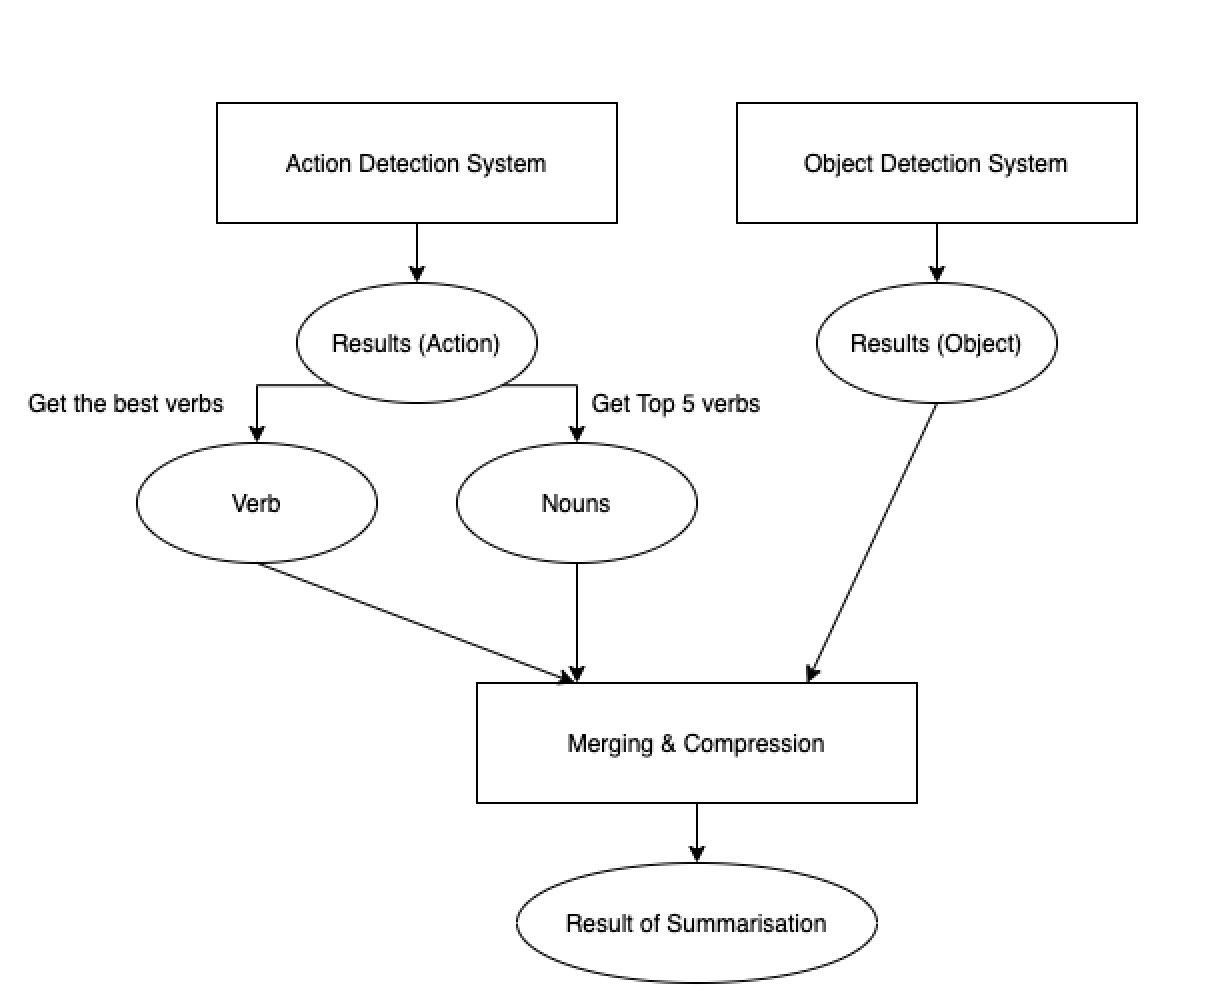
\includegraphics[scale=0.4]{imgs/PlannedFlow.png}
    \caption{A diagram that shows the planned flow of the video summarisation system}
    \label{fig:planned_flow}
\end{figure}

The image above shows the planned flow of the video summarisation system that I designed. Firstly, the video summarisation system uses the action detection system and object detection system to extract corresponding data from video frames. The action detection system will divide the target video into multiple segments for every 1 second of the video, and get a verb and 5 nouns for each video segment. Similarly, the object detection system will detect objects from the video frames of every 1 second of video.

After extracting data from video frames, the system will execute the merging process that merges the intermediate results that are generated by each detection system. By using the result of the merging process, the system will start summarising the video by compressing the merged results. When the compression finishes, the system will generate the final output.

\subsection{Object Detection}

Object Detection is a computer technology related to computer vision and image processing that deals with detecting instances of semantic objects of a certain class in digital images and videos. Object Detection has applications in many areas of computer vision, including image retrieval and video surveillance. Also, Object Detection has been used for many machine learning and deep learning projects, such as face recognition or object tracking.

The \hyperlink{ref14}{object tracking system [14]} is a component that keeps track on the object by watching the stream of images. As you know the video is a stream of frames and audio data. Therefore, it would be possible to say that the system could find the keyframes from the video by using the system that works similarly with the object tracking system by detecting the objects from the frames of the video. Hence, one of the main components of this project would be the object detection system, which detects the objects' names and coordinates from each frame, which will be used for finding the keyframes.

\subsubsection{Object Detection - YOLOv3}

"YOLO", which stands for You Only Look Once, is a real-time object detection system that is one of the most widely used object detection models. In this project, the YOLOv3 model is used to detect the objects in each frame of the video. According to the \hyperlink{ref2}{J. Redmon et al. [2]}, the YOLOv3 guarantees to detect objects within reasonable execution time.

In general, most detection systems repurpose classifiers or localizers to perform detection. Those detection systems apply the model to an image at multiple locations and scales, and consider the high scoring regions of the image as detections. However, the YOLO model uses a different approach. According to \hyperlink{ref2}{J. Redmon et al. [2]}, YOLO applies a single neural network to the full image. This network divides the image into regions and predicts bounding boxes and probabilities for each region. These bounding boxes are weighted by the predicted probabilities. By doing this, the YOLO model has several advantages over classifier-based systems. Firstly, the predictions are informed by the global context in the image, since the YOLO model looks at the whole image at test time. Moreover, the YOLO makes predictions with a single network evaluation unlike the R-CNN model, which requires thousands of networks for a single image.

Basically, the YOLOv3 makes the predictions to find the bounding boxes. For each bounding box, the YOLOv3 model uses the multi-label classification to predict the class that the given bounding box may contain. While making the prediction, the YOLOv3 model uses the feature extractor, which has several convolutional layers, to extract the features from each bounding box. By using the extracted features, it predicts to find the class that is most suitable to the given bounding box, and return the name of the detected object and the coordinates of the bounding box. By using this algorithm, the YOLOv3 could detect objects in the image within a short time with fairly good accuracy.

As the main aim of this project is not implementing the YOLOv3, but using it for the video summarization system, I used \hyperlink{ref15}{the existing PyTorch implementation of the YOLOv3 [15]}. The default pretrained YOLO model is trained with the COCO dataset. COCO is a large-scale object detection, segmentation, and captioning dataset. It is most widely used dataset for the object detection projects, since it contains more than 330,000 images with 80 different types of objects. However, as the COCO dataset only contains 80 different types of objects, the YOLO model was not able to detect most foods and utensils in the cooking video.

\subsubsection{Retraining the YOLOv3}

As the YOLOv3 model with the COCO dataset could only detect 80 different kinds of objects, the accuracy of the YOLOv3 model for detecting food instances from cooking video was much lower than expected. For example, the YOLOv3 gives the "toilet" label to the white doughnut. This is because the YOLOv3 is too generic and needs to be retrained with specific image dataset with foods. Thus, I had to retrain the YOLO model.

It is clear that the usual difficulty with the Deep Learning is the requirement of a large dataset. Instead of investing great labor to collect the required food images, I decided to retrain the YOLO with the \hyperlink{ref4}{Food100 dataset [4]} and \hyperlink{ref7}{Edinburgh Utensils dataset [7]}.

The Food100 dataset contains 100 classes of food photos, where there are more than 100 images for each class. Each food photo has a bounding box indicating the location of the food item in the photo. Also, the dataset contains the label files for all classes, which contains the coordinates of the bounding boxes and the names of the object in each bounding box. Henceforth, it would be possible to say that the Food-100 is a perfect dataset to retrain the YOLO model to detect foods in the video.

The Edinburgh Utensils dataset contains 20 classes, where each class contains more than 20 images. This dataset only contains 897 images, which is not big enough. If the number of data is too small, it might be possible that the retrained model is not fitted well. To overcome this problem, I increased the number of images by doing the image augmentation (resize, flip and rotate images). Unlike Food100 dataset, Edinburgh Utensils dataset only contains the raw images of kitchens utensils. Thus, to use it for retraining YOLO, the images should be labelled with suitable format. To solve this issue, the \hyperlink{ref21}{YOLO annotation tool [21]} was used.

To retrain the YOLO model, the DarkNet, which is the original implementation of the YOLO model, is required. You could download and install the DarkNet by following the instructions in the \hyperlink{ref5}{DarkNet website [5]}. After installing the DarkNet, we need to start preparing the YOLO training process. To get Darknet YOLO training to work, several things are required - 1) Object bounding box file for each image, 2) Class name file for all the category names, 3) Training dataset file for the list of training images, 4) Validating dataset file for the list of validating images, 5) Configuration file for YOLO neural network specification, and 6) Data location file for finding all the data information. Since the Food100 dataset provides the bounding box file and the class name files, all we need to do for the YOLO training are task 3), 4), 5) and 6).

For the task 3) and 4), DarkNet requires the text files called "train.txt" and "test.txt", where "train.txt" file contains the list of file paths of the files that will be used for the training, and "test.txt" file contains the list of file paths that will be used for the testing. To generate these text files, I wrote a simple python script, which reads the label files that the Food100 dataset provides, and splits all Food100 class images into "train.txt" training image list and "test.txt" validating image list. When splitting the data into train and test set, the ratio of train set and test set is 8 : 2, which means that using 80\% of dataset as training dataset and using 20\% of dataset for testing.

The configuration file contains the specification of the YOLOv3 neural network. Since the target dataset has been changed, the content of the configuration file also need to be changed. To use the retrained YOLO model, the new configuration file should be created. The contents of the new configuration file should be almost same with the contents of the original configuration file, as both of them are using the YOLOv3 model. However, the number of filters of some layers and the number of classes should be modified, since the number of classes of the Food-100 dataset is different with the coco dataset. According to the \hyperlink{ref2}{YOLOv3 paper[2]}, the number of filters is equal n is $$n = (a + b + 1) * 3$$, where a is the number of classes and b is the number of the coordinates. Since the value of the n in the default configuration file is 245 (245 = (80 + 4 + 1) * 3 = 85 * 3  (a = 80, b = 4)), the value of the n in the new configuration file should be 315 ((100 + 4 + 1) * 3 = 105 * 3 = 315) for the Food100 dataset, and 75((20 + 4 + 1) * 3 = 25 * 3 = 75) for the Edinburgh Utensils dataset. Thus, by replacing the number of classes and filters with suitable numbers, a new configuration file for the custom dataset will be generated.

To retrain the network, the programmer should let the Darknet know the file paths of the label files, because the DarkNet does not know where the label files, text files ("train.txt" and "text.txt"), and class name file are located in. Thus, the data file, which tells the DarkNet the file paths of those files, should be created before running the DarkNet to retrain the YOLOv3 model with the custom data. All the things that should be done in this step are finding the image files, creating label file for each class, and splitting the set of images into train set and test set.

When training the neural network, both cases of under-fitting and over-fitting should be considered, as both of them could bring serious problems to the neural network. To avoid both overfitting and underfitting, the retraining process should iterate the suitable number of epochs. Basically, the DarkNet recommends retraining the YOLO model by iterating at least 500 epochs for each class. Thus, we will iterate 50,000 iterations for Food100 dataset, and 10,000 epochs for the Edinburgh Utensils dataset.

When retraining the YOLOv3 model, the programmer could choose either YOLOv3 or YOLOv3-tiny to use.As the name depicts, the tiny model is a tiny YOLO model, which is much smaller than the general YOLO model. With the YOLO-tiny model, the retraining process could be finished sooner, however, the accuracy of the YOLO-tiny model is not as good as the general YOLO model.

Similarly, the programmer could choose to retrain last N layers only, or retrain the model with fine tuning. The fine tuning is a retraning method that retrains half of the layers that the YOLO model contains. So, by retraining last 1 layer of the YOLO-tiny model, it would be possible to retrain the neural net extremely faster than fine tuning the YOLO model. However, then the accuracy of the retrained model will be definitely lower than the fine tuned YOLO model.

To understand the semantics of the video correctly, the accuracy of the object detection system should be good enough for finding the keyframes. As a result of the video summarization system strongly depends on the result of YOLOv3, it would be better to choose the accuracy rather than training speed. Henceforth, it is possible to say that retraining the YOLOv3 model with fine-tuning is more suitable for this project than retraining the YOLOv3-tiny model or retraining the last N layers only.

By executing the command "./darknet detector train (\textit{data file path}) (\textit{config file path}) (\textit{weights file path})", the DarkNet program will start the retraining process for the YOLOv3 model. For every 100 epochs, the DarkNet automatically stores the backup weight files in the backup directory, thus, even if the program terminates in the middle of the retraining process, it would be possible to restart the retraining process from the certain point.

Once the retraining process terminates, rename the latest backup weights file with the suitable name (i.e. food100\_final.weights). By using the generated weights file and the corresponding name file and configuration file, now the object detection system could detect the food objects from the images.

After finishing the training processs, all models were evaluated by using the confusion matrix function of scikit-learn. And it was found that the accuracy of the model that is retrained with Edinburgh Utensils dataset is too low. Fortunately, the action detection system provides nouns, and the basic YOLO model covers several important utensils such as pot, pan, and knife. Thus, it was decided to replace the utensil model with the action detection system's noun detecting component and basic YOLO model. The result of the evaluation of retrained YOLO models will be explained in detail in the \hyperlink{evaluate_yolo_with_cm}{"Confusion Matrix of retrained YOLO models"} section.

\subsubsection{Merging the sets of detected objects}

As mentioned above, the object detection system uses 2 YOLO models - one with the COCO dataset, and the other with the Food100 dataset. So, the YOLO COCO model will return the list of general objects that are included in the COCO dataset, where the YOLO Food100 model will return the list of food objects that are included in the Food100 dataset.

The main reason that I did not retrained the model with both Food100 and COCO dataset is because the number of images for each class in COCO dataset and Food100 dataset are different. Basically, the Food100 dataset only has about 150 images for each class, however, the COCO dataset contains more than 500 images for each class. Due to this difference, the retrained model that is retrained with both COCO dataset and Food100 dataset was not able to make a correct prediction for the food object. Furthermore, since the size of the COCO dataset is too big, the retraining process took too much time. Apparently, one of the most attractive points of the YOLO is it's short retraining time. Thus, it might be possible to say that there is no merit if the retraining process takes too much computational resources. Henceforth, I decided to retrain the YOLO model with just Food100 dataset, and make new functions that merges the outputs of original YOLO model and food YOLO model.

When the system detects the object, the system stores the 2 coordinates and label name of each bounding box. Then, by using those coordinates, it calculates the middle point of the bounding box and the euclidean distance between 2 coordinates, which is identical to the length of the diagonal of the bounding box. 

\[the\_length\_of\_diagonal = \sqrt{((x2 - x1)^{2} + (y2 - y1)^{2})}\]

And when the system merges the output lists, it first compare all middle points and length of the diagonals of all detected objects to check if there are any duplication. If not, the system will just merge the output lists. However, if the system founds the duplication, then the system will first compare the label name of 2 objects. If the label names are same, then it would be easy to merge the outputs. On the other hand, if the label names are not same, then the system should determine which object to use.

To overcome the issue mentioned above, the object detection system checks the confidence value that each YOLO model returns. Basically, the YOLO gives a float type constant as a confidence value between 0 and 1. This value depicts how much the YOLO is confident with the prediction that it made. For example, if the YOLO gives 0.3 as a confidence value, then that means that the YOLO is 30\% sure with the prediction that it made. Similarly, if the confidence value is 0.8, then that means that the YOLO is 80\% sure with the prediction that it made. However, it is clear that the confidence value is not an accuracy. This means that even if the YOLO is confident with the prediction that it made, that does not mean that the prediction is accurate. So, when merging the output lists, the system should check multiple conditions.

If confidence value of both general object and food object are higher than the 0.5, then the system will choose the general object. And if the confidence value of the general object is higher than 0.5, however, the food object's confidence value is less than 0.5, the system will choose the general object. Similarly, if the confidence value of the food object is higher than 0.5, however, the general object's confidence value is less than 0.5, then the system will choose the food object. If the confidence of both COCO object and food object are less than 0.5, then the system will ignore them.

\subsubsection{Selecting frames that are used for object detection}

Initially, the object detection system was doing object detection for every frame in the video. However, the object detection system took more than 1 hour to process a 2-minute long video. The main reason for the long execution time of the object detection system was that the YOLOv3 takes 2 ~ 3 seconds for detecting objects in a frame. Since the YOLOv3 itself takes more than 2 seconds for processing a single frame, the object detection took much more time than I expected to detect objects from video frames. For example, if the fps of the target video has a total of 2400 frames (2-minute video with 20 fps), then the total running time of the object detection would be at least 4800 seconds. In other words, the object detection system requires at least 1 hour and 20 minutes to process this video.

Apparently, 80 minutes for processing the 2-minute video is not ideal. To overcome this problem, I made the object detection system to execute object detection for every frame corresponding to 1 second of the video. For instance, if the fps of the target video is 30, then the system will first perform the object detection for the first frame, and the object detection system will execute the object detection when it gets the 31st frame. So, the system will perform the object detection for every 30 frames, which corresponds to 1 second in the target video. By using this method, it was able to reduce the total execution time of the object detection system.

\subsection{Action Detection}

It is clear that the object detection is not enough for implementing the video summarization system, because it is almost impossible to understand the semantic of the video. Since the video is a stream of frames, the video summarization program should be able to understand the relationship between each frame to find the key frames. To make the system to understand the video, I decided to add the action detection system as a sub-system. By detecting the action, it would be possible to understand the semantic of the current frame, which is definitely helpful for the video summarization system to choose the key frames.

Again, to detect the action, a video dataset was required, whose size is huge enough. Also, the domain of the videos should be related to the cooking, otherwise, it would be hard to detect actions from the cooking videos. After spending several days to find the dataset to use, I was able to find the open sourced dataset with the pre-trained model, which is called \hyperlink{ref8}{"Epic Kitchens" [8]}.

\subsubsection{Action detection models - Epic Kitchens}

The \hyperlink{ref8}{"Epic Kitchens" [8]} is an open sourced dataset, which contains the videos with first-person vision. The videos in this dataset depict non-scripted daily activities. Basically, this dataset is  a large-scale egocentric video benchmark recorded by 32 participants in their native kitchen environments. All participants are asked to start recording every time they entered their kitchen until they finished using their kitchen. Also, for the annotation, participants were asked to narrate their own videos, so that they could reflect true intention. According to their \hyperlink{ref12}{paper [12]}, they describe their object, action and anticipation challenges, and evaluate several baselines over two test splits, seen and unseen kitchens. Also, the \hyperlink{ref8}{"Epic Kitchens" [8]} provides the pre-trained models by using the PyTorch Hub, which will be discussed in the \hyperlink{actionDetection_used}{"Technologies Used"} section.

The Epic Kitchens provides a set of pre-trained models where each of those models uses different action detection algorithm. The provided models are \hyperlink{ref16}{TSN (Temporal Segment Networks) [16]}, \hyperlink{ref13}{TRN (Temporal Relational Reasoning) [13]}, and \hyperlink{ref17}{TSM (Temporal Shift Module) [17]} based networks, including a variety of their variants.

\hyperlink{ref16}{Temporal Segment Networks [16]} is a model that propagates each snippet through a 2D CNN backbone and aggregate the class scores across segments through average or max pooling. As a consequence, TSN is unable to learn temporal correlations across segments. TSN is typically trained on RGB and optical flow modalities and combined by late-fusion.

Similarly, \hyperlink{ref13}{Temporal Relational Reasoning [13]} propagate snippets through a 2D CNN, like in TSN, up to the preclassification layer. These produce features rather than class confidence scores. In order to support inter-segment temporal modelling, these segment-level features are then processed by a modified relational module [8] sensitive to item ordering. Two variants of the TRN module exists: a single scale version which computes a single n-segment relation, and a multi-scale (M-TRN) variant which computes relations over ordered sets of segment features of size 2 to n. Once the relational features have been computed, they are summed and fed to a classification layer.

\hyperlink{ref17}{J. Lin et al. [17]} stated that "TSM based networks functionally operate just like TSN, snippets are sampled per segment, propagated through the backbone, and then averaged". Unlike TSN, the backbone of the TSM network is modified to support reasoning across segments by shifting a proportion of the filter responses across the temporal dimension. This opens the possibility for subsequent convolutional layers to learn temporal correlations.

By passing multiple frames, the pretrained models will detect the action in those frames, and convert the array of frames to the features. When extracting the features, the pretrained models will return 2 types of features - one for the verbs and one for the nouns. The the each extracted feature could be converted to the corresponding logits. By using the Softmax function as an activation function, the action detection system will calculate the mean of the given logits. The result of the calculation will be a list that contains the indexes and probabilities of labels. Since the action detecting models returned 2 logits (1 for verbs and the other for nouns) the system could calculate and return lists of indexes and probability values for nouns and verbs.

\subsubsection{Top K nouns and verbs}

Each of 3 action detection models will return 4 lists (probability values of nouns, probability values of verbs, indexes of verbs, and indexes of nouns), thus, now the system has total 12 lists. All 3 of these models are trained with 126 verbs and 351 nouns. However, since the main of this action detection system is to detect the motion and return suitable verbs and nouns that depicts the detected action, the video summarization system only requires 1 verb and 1 noun. Henceforth, the action detection subsystem should be able to choose the best verb and the best noun.

According to \hyperlink{ref8}{D. Damen et al. [8]}, the accuracy of the noun prediction is lower than the verb prediction, thus, it is recommended to use Top5 nouns rather than using the best noun for the noun prediction, which might be possible to increase the accuracy of the noun prediction. Due to this reason, it was decided to make the action detection system to use Top 5 nouns for detection action from a segment of video frames rather than using the best noun. In other words, each action detection model will return 1 verb and 5 nouns for every iteration.

\subsubsection{Merging outputs from each action detection models}

Each pretrained model in the action detection system will return 5 nouns for the input frames, which are the frames for 1 second of video. As there are 3 pretrained models, 15 nouns will be returned. Clearly, there would be some intersection between 3 sets of nouns. So, we could decrease the number of returned nouns by removing the duplicating nouns. Also, we could decrease the number of nouns by filtering the most irrelevant nouns by using the \hyperlink{ref24}{wordnet [24]}.

The \hyperlink{ref24}{wordnet [24]} is a lexical database of semantic relations between words. This means that by using the wordnet, it would be possible to find the most irrelevant words by calculating the simularity values between returned nouns. So, what I designed the action detection system to calculate the sum of similarity values between each noun and all other nouns, and find the noun that has the smallest similarity value. By using this method, the action detection is able to filter the most irrelevant word, so that the action detection system could decrease the number of detected nouns.

\subsubsection{Action detection with OpenCV and scikit-video}

While implementing the Action detection system with OpenCV, I found that the VideoCapture object of the OpenCV-python library fails to reads some files. According to the \hyperlink{ref22}{github issue page [22]}, this error is a well-known error, which was occurred from OpenCV-python version 3, where the version that I am using is OpenCV-python version 4. Basically, the VideoCapture object fails to read more than 1 second of video if the encoding method or codec that the target video uses are not supported by the OpenCV-python library. For example, if the MP4 file uses Timecode as a codec, then the VideoCapture fails to read frames from the file after reading 1 second of video.

To fix this issue, I made used the scikit-video library. Basically, the scikit-video uses the \hyperlink{ref23}{ffmpeg command line tool [23]}, which makes the action detection system possible to reads the frames from the video even if the target file uses some codec or encoding method that are not supported by the OpenCV library.

So, the action detection system will first run the OpenCV version to detect actions from the video frames. And if the OpenCV fails to read the video file, then the scikit-video version to detect actions from the video frames.

\subsection{Merging the sub-systems}

After detecting actions and objects from the target video, the video summarization system should merge the results of action detection and object detection. Then, the system should compress the result to summarize the video.

\subsubsection{Filtering the most irrelevant words}

Apparently, there is a possibility that the results of action detection system and object detection system might contain unnecessary words, which will make the system hard to summarise the video. To overcome this issue, the \hyperlink{ref24}{wordnet [24]} was used. Again, by using the wordnet, the system will calculate the similarity value between each word, and find words that are irrelevant to other words.

When using the wordnet for merging the results of the action detection system, the program just compares the sum of similarity values between each noun and all other nouns. However, at this time, there are some constraints that make the problem much complex. First, we need to find out the most irrelevant nouns and objects by comparing the sum of similarity values between verbs and nouns, nouns and objects, and verbs and objects. Second, when filtering the words by similarity values, the suitable threshold value would be required, which will help the system to filter irrelevant words.

To fulfil those requirements, I designed the system to generate the lists of combinations for each of verbs and nouns, verbs and objects, and nouns and objects. Each list will contain tuples, which represent the combination. For example, the first list will contain tuples, where each tuple is constructed with verb and noun. Similarly, the second list will contains tuples of verbs and objects, and the third list will contain the tuples of nouns and objects. By iterating each combination list, the program would be able to calculate the similarity values. After calculating the similarity values, the system will find the biggest similarity value. Then, the program will calculate the threshold value by divide the biggest similarity value by 2.

\[threshold = max(similairty\_values) / 2\]

The calculated threshold value will be used for filtering the words that have smaller similarity value than the threshold. By applying this method to all 3 lists, the system could filter irrelevant words from the result words.

\begin{figure}[H]
    \centering
    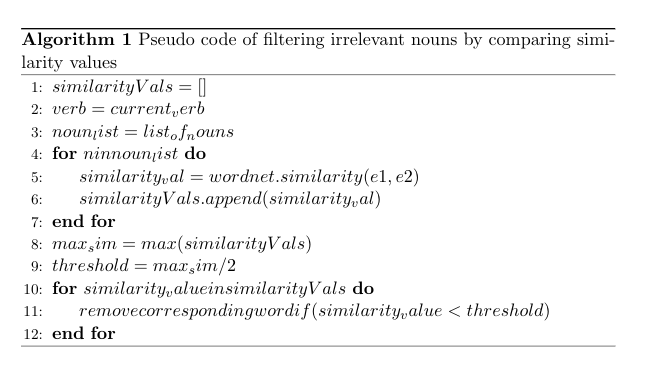
\includegraphics[scale=1]{imgs/pseudo_code.png}
    \label{fig:pseudocode_merging}
\end{figure}

The pseudo code above shows the algorithm that filters all irrelevant nouns by comparing the similarity values between each noun and verb. The system will apply same algorithm to nouns and objects, and verbs and objects.

\subsubsection{Compressing the results}

To compress the results of merging process, the system will compare verbs, nouns, and objects to find the meaningful changes. First, the system will iterate the list of results, where each element of result list is an object that contains 1) the best detected verb, 2) list of detected nouns, 3) list of detected objects, and 4) frame number. Then, the system will compare current verb, nouns, and objects with the previous verb, nouns, and objects.

The hardest part of designing the compression method was defining the criteria of the meaningful change points. The most straightforward way would be just make the system to find if any of verb, nouns, and objects are changed. Clearly, this method will be able to summarise the video if and only if the action detection system and the object detection system never make wrong decisions. The algorithm that finds the meaningful change points should compress the results well, so that the summarised video does not contain more frames than necessary. So, I had to be careful for designing the key frame selection algorithm.

After a long troubled time, I designed the key frame selection algorithm to check if either 1) more than 60\% of nouns are changed when the verb is changed or 2) more than 80\% of nouns are changed when more than 40\% of objects are changed. To implement this algorithm, I made the system to find the intersection of 2 lists (lists of nouns or objects). When the system calculates the intersection, it will compare the length of the intersection list with the corresponding threshold value. The threshold value is calculated by multiplying the length of the previous list with the corresponding percentage value (one of 0.6, 0.4, and 0.8).

If the system considers the current frame as a key frame, then the system will store the frame number of the current frame in the result list, and record the data of current frame in the text file. Each line in the generated text file will contain time string, verb, list of nouns, and list of objects. To record the time, the compression system will convert the frame number to the corresponding time string by division with fps value of the original video file. The format of the converted time string will be either 'mm:ss' or 'hh:mm:ss'. The system will determine the time string format by checking the total time of the video. So, if the total time of the video is less than 1 hour, then the system will use the 'mm:ss' format for the time string. And if the total time of the video is greater than or equal to 1 hour, then the system will use the 'hh:mm:ss' format for the time string.

After creating the text file of results of the compression, the system will generate the summarised video. To generate this video, the system will find every key frame, and extract F frames from the video, where F is equal to fps of the video. The main reason of rebuilding the video with F frames for each key frame is to generate the understandable video. If the system only uses the key frames for rebuilding the result video, then it will be impossible for people to watch the video. As the video that is rebuilt with key frames only contains K frames, where K is the number of all key frames, the video playback speed will be too fast, which might make it impossible for people to understand what is actually going on in the video frames. To overcome this issue, the system that I designed reads F frames from the original video for each key frame, and rebuild the result video by using those read frames. By doing this, the fps of the result video would be equal to the fps of the original video. Henceforth, as far as the original video is human watchable and understandable thing, people would be able to watch and understand the summarised video.

When generating the result video, the scikit-video was used, because of the codec issue of the OpenCV-python library that I mentioned above. Since the scikit-video uses the ffmpeg internally, the ffmpeg should be installed in the machine before running the compression process.


\section{Results and Discussion}

\subsection{Comparison with DOER}

When writing the DOER report, I was planning to implement the video summarisation system by using object detection and frame comparison method. However, while having the research, it was found that designing the video summarisation system with frame comparison would be too hard for the SH project. Furthermore, while having research about YOLOv3 model, I realised that using the YOLOv3 model would not be good enough to extract data that helps the system to understand and summarise the video. Henceforth, I changed the design of the video summarisation system to use action detection model with the object detection system to extract more data from video frames.

\subsection{Evaluation}

\subsubsection{Evaluation for the retrained YOLOv3 models}

\hypertarget{evaluate_yolo_with_cm}{A confusion matrix} is a table that is often used to describe the performance of a classification model on a set of test data for which the true values are known. It allows the visualization of the performance of an algorithm. To evaluate the accuracy of retrained YOLO models, the confusion matrix is used.

\begin{figure}[H]
    \centering
    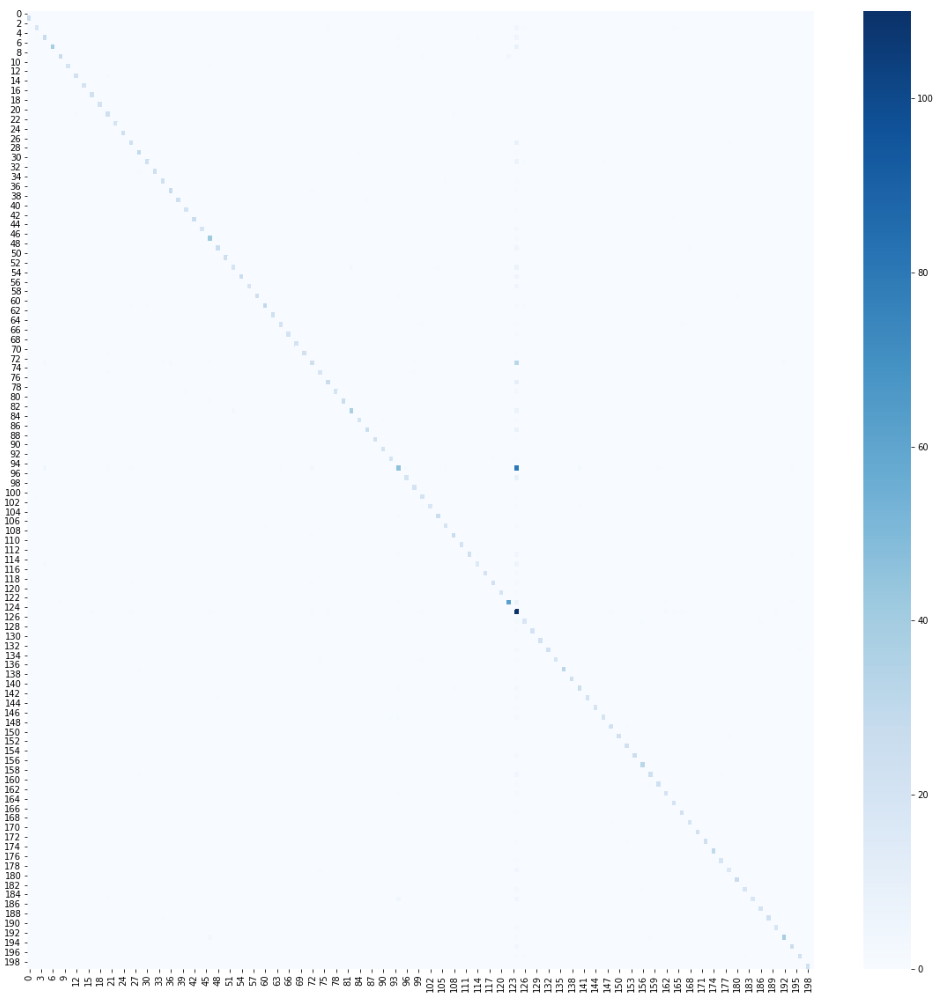
\includegraphics[scale=0.6]{imgs/cm_food100.png}
    \caption{Confusion Matrix of YOLO model with Food100 dataset}
    \label{fig:cm_food100}
\end{figure}

The image above shows the confusion matrix of the YOLO model that is retrained with the Food100 dataset. As the confusion matrix shows, the YOLO model is well trained.

To further understand the accuracy of the YOLOv3 model that is retrained with the Food100 dataset, I look the confusion amongst the top 10 most frequent classes in the Food100 dataset. To implement this confusion matrix, I replaced the top 90 most infrequent classes, which are not included in the top 10 most frequent classes, with 'other'. The figure \ref{fig:cm_food100_top10_classes} shows the confusion matrix, and the table below shows the TP, TN, FP, and FN values of each TOP 10 class of the food classification model.

\begin{figure}[H]
    \centering
    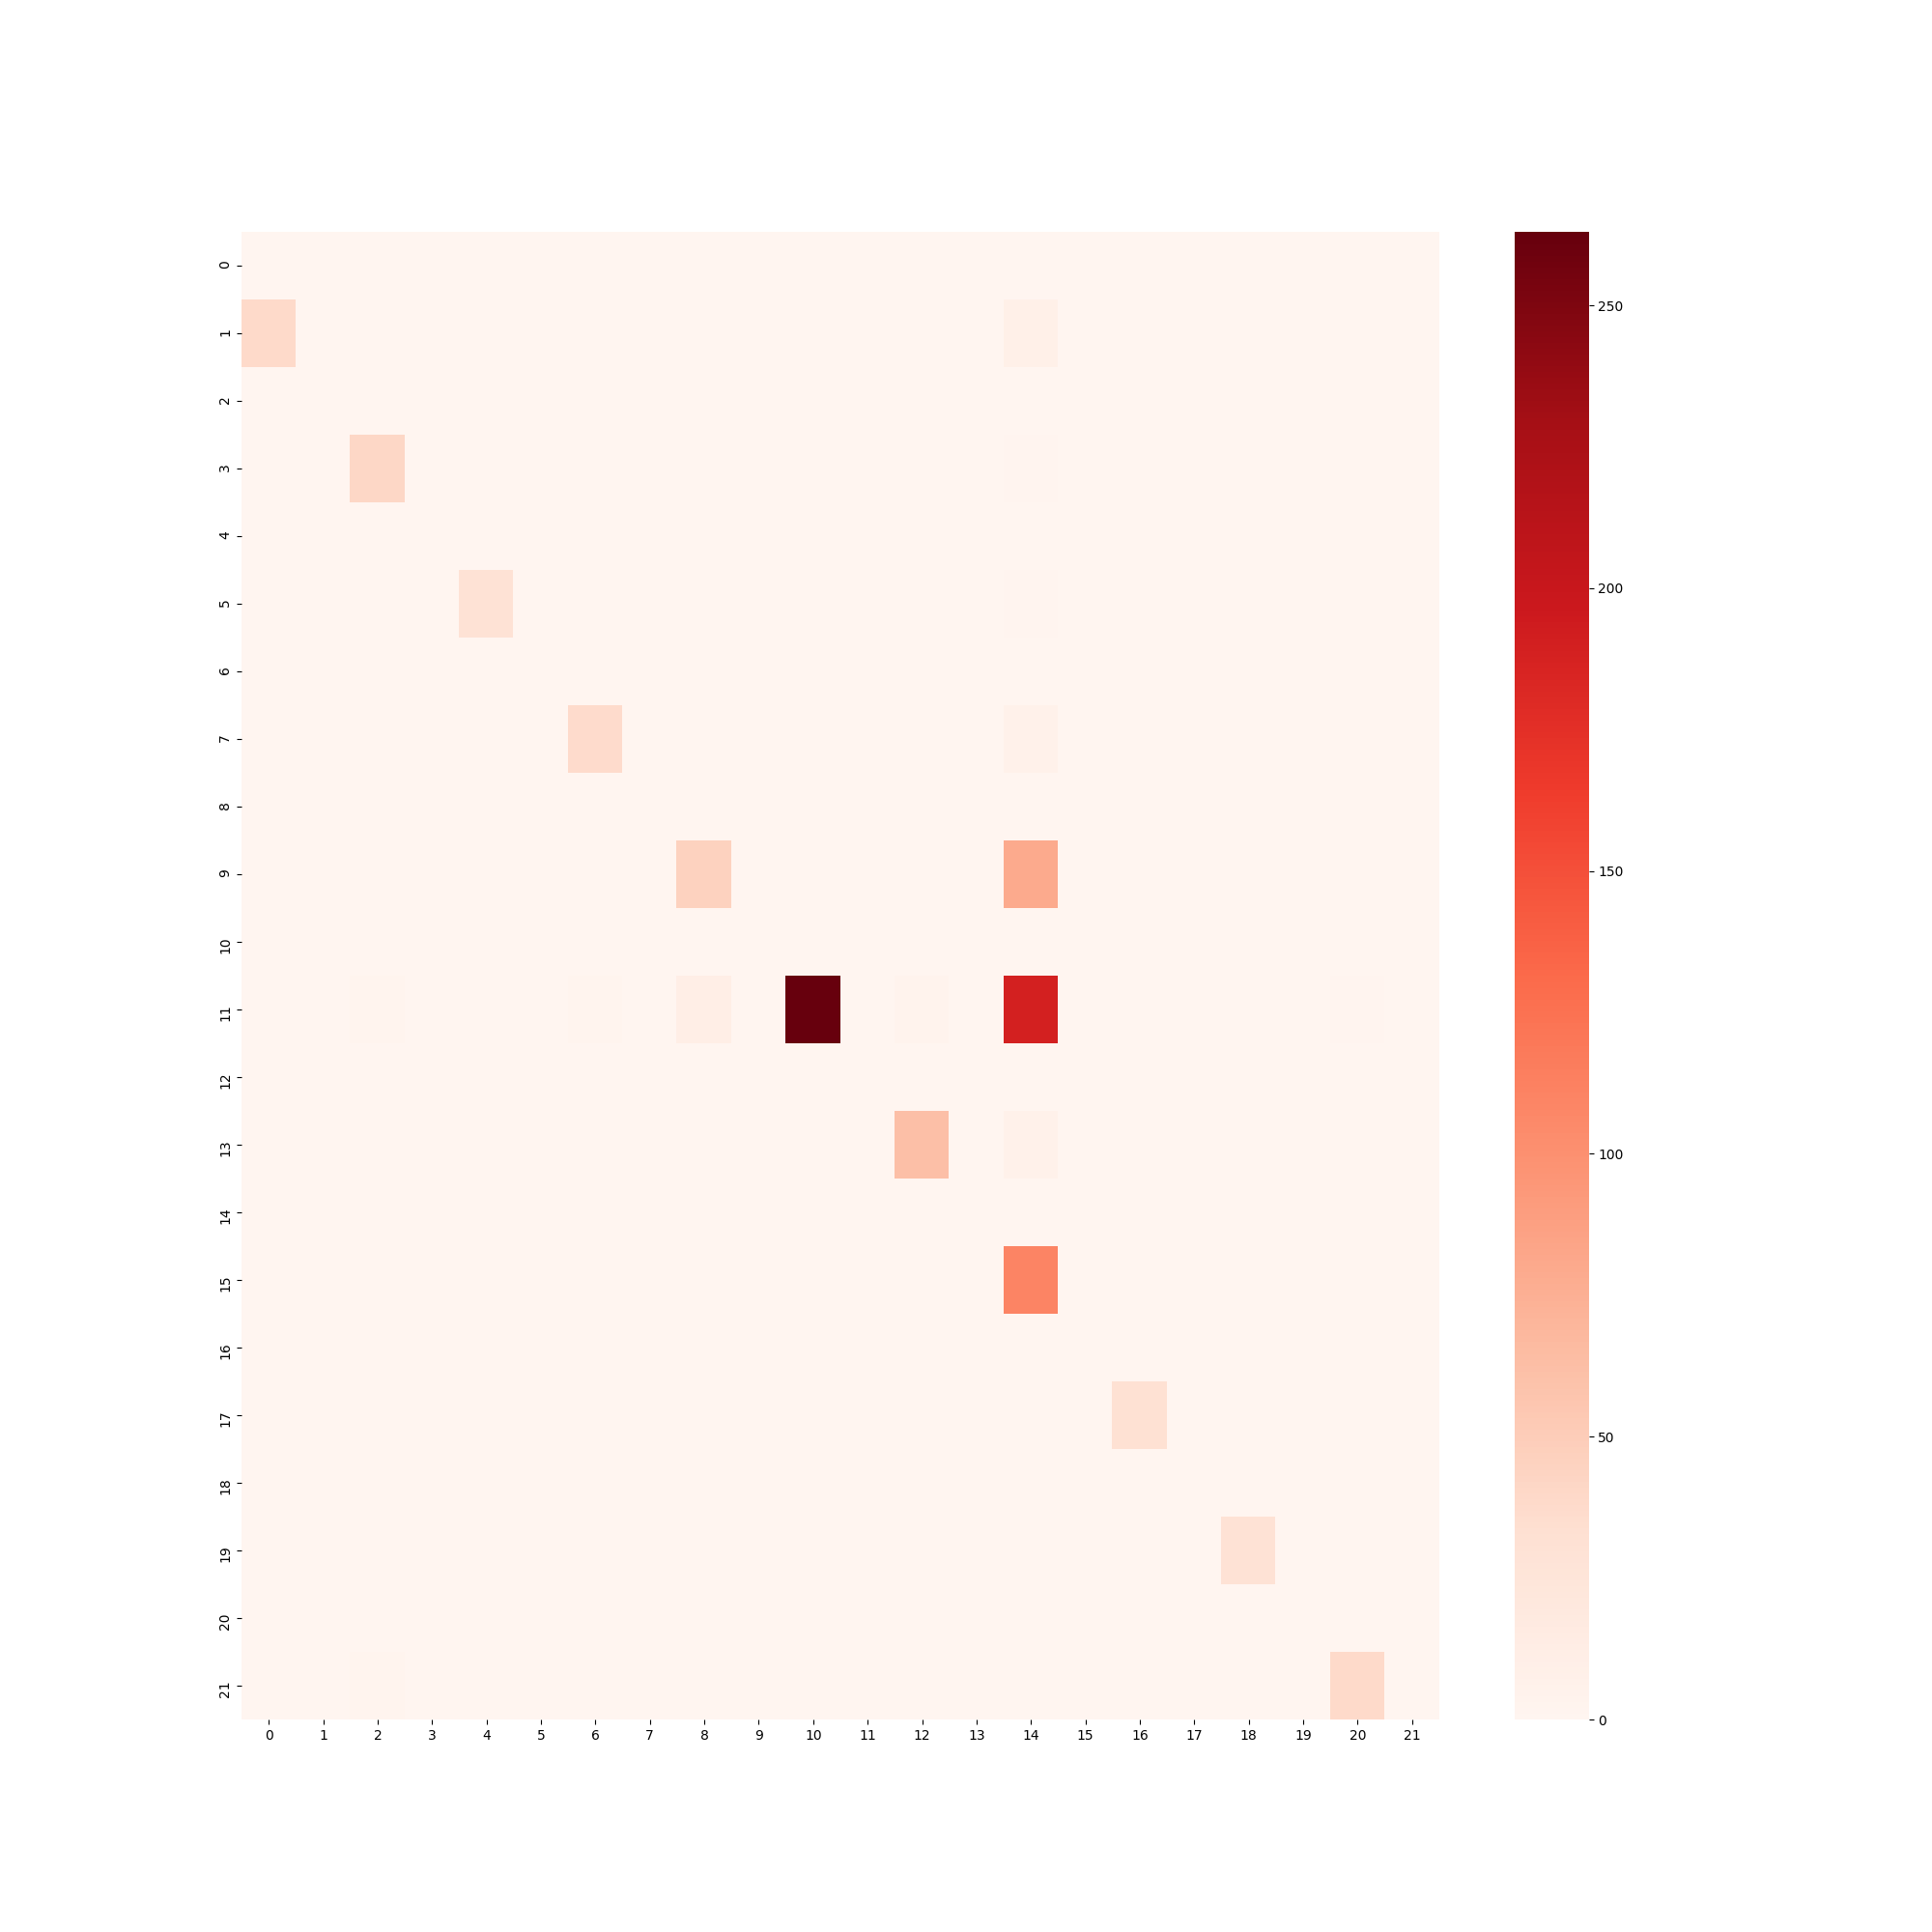
\includegraphics[scale=0.2]{imgs/confusionMatrix_food_modified.png}
    \caption{Confusion Matrix of YOLO model with Top 10 classes of Food100 dataset}
    \label{fig:cm_food100_top10_classes}
\end{figure}

\begin{figure}[H]
    \centering
    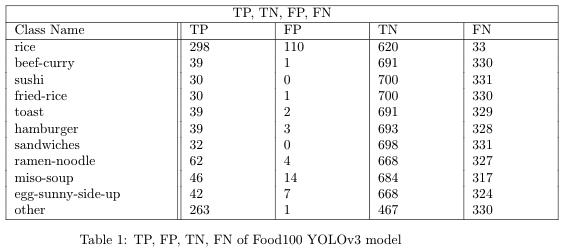
\includegraphics[scale=0.5]{imgs/Food100_table.png}
    \label{fig:food100_table}
\end{figure}

As the table above shows, the values of TP and TN are greater than the corresponding values of FP and FN. Therefore, it would be possible to say that the predictions that are made by the YOLOv3 model that is retrained with the Food100 dataset are generally accurate. Also, as you could see in the figure \ref{fig:cm_food100}, the model works fine for all classes. Thus, I decided to use this model for the video summarisation system.

Unlike the food YOLOv3 model, the YOLOv3 model that is retrained with the Edinburgh Utensils dataset did not trained well. Below is the confusion matrix of the YOLOv3 model that is retrained the Edinburgh Utensils dataset.

\begin{figure}[H]
    \centering
    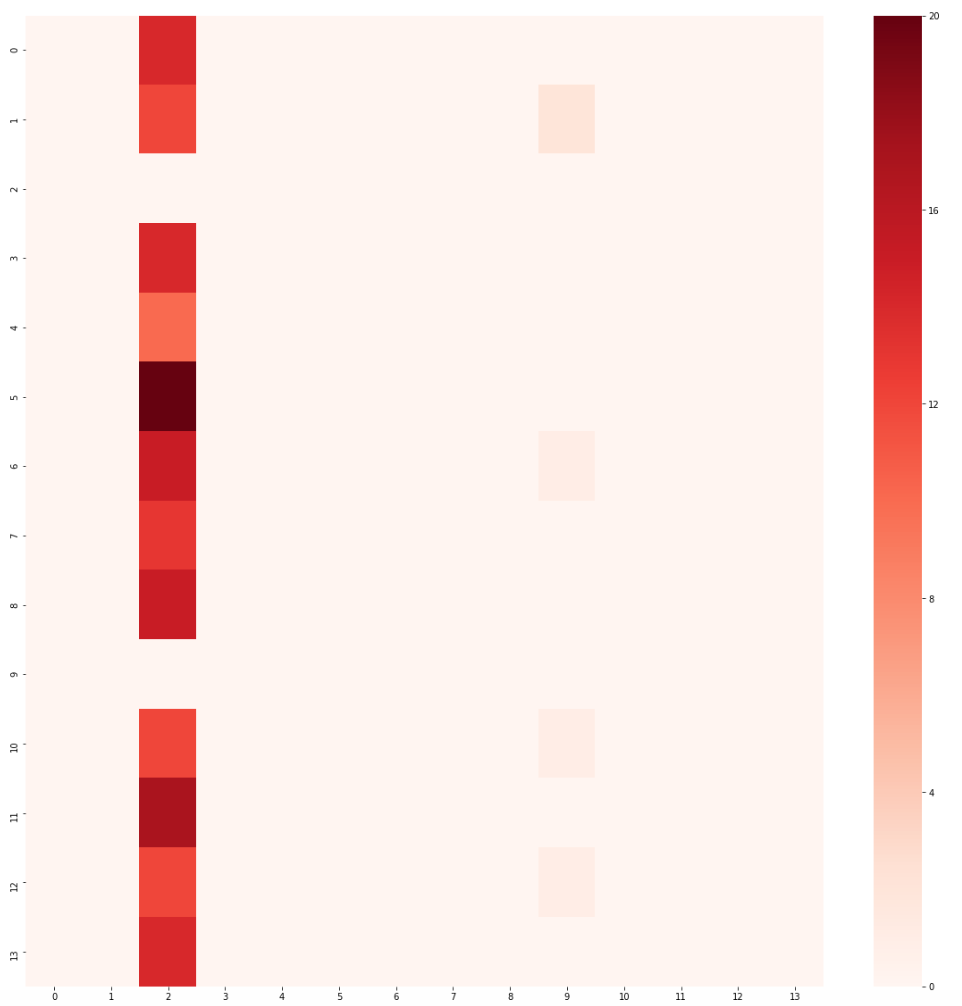
\includegraphics[scale=0.4]{imgs/cm_utensils.png}
    \caption{Confusion Matrix of YOLO model with Edinburgh Utensils dataset}
    \label{fig:cm_food100}
\end{figure}

As you could see in the image above, the predicted values are biased for some reason. Perhaps, this is because that I made some mistake whild doing the data augmentation methods that I applied for the Edinburgh Utensils dataset. As I mentioned in the Design and Implementation section, I decided to use the data augmentation to increase the number of images for each class. Basically, I flipped vertically the image, and rotate the images by $n * \pi / 6$ (n = 1 .. 5). And I am assuming that the rotated images made the model confused to classify utensils, which affected to the accuracy of the utensil classification model. Due to the time limit, I was not able to restart the retraining process, so I was not able to find the actual problem that decrease the accuracy of the utensil classification YOLOv3 model.

Fortunately, the original YOLO model covers some kitchen utensils, and the action detection system detects the noun for the action. Henceforth, rather than keep retraining the YOLO model until it works properly, it was decided that combining the result of general YOLO model and the nouns that are detected by the action detection system.

\subsubsection{Evaluation for the action detection system}

To evaluate the performance of the action detection system, the testing set of the Epic-Kitchens dataset, which contains the videos that the action detection models never have seen while training process, was used. For all TSN, TRN, and TSM models, the ResNet-50 backbone was used with the RGB counterparts.

According to \hyperlink{ref8}{D. Damen et. al. [8]}, the verb classification relies on temporal modelling, however, the noun classification does not rely on the temporal modelling as much since objects can be recognised from a single frame. Thus, initially, I was planning to compare the performance and accuracy of verb classification for each TSM, TRN, and TSN with different backbone. However, I found that the provided pretrained model does not support BN-Inception backbone for some models, thus, I decided to keep using the ResNet-50 as a backbone for all 3 models for the consistency.

As you could see in the figure \ref{fig:chartForEvalActionDetection}, for the verb classification, the accuracy of the TSN is much lower than the accuracy of TRN and TSM. Here, it would be possible to say that the TSM and TRN extracts temporal relational information much better than the TSN model. Also, you could find that the TSM and TSN perform the best on the noun classification task, with TRN models lagging about 3\% points behind. A possible explanation for the observed drop is that the relation module within TRN places heavy emphasis on extracting temporal relational information, which is of little relevance in recognising objects. Thus, it would be possible to say that the TRN relies heavily on extracting temporal relational information, so that the TRN works the best on the verb classification, but does not work well on the noun classification.

\begin{figure}[H]
    \centering
    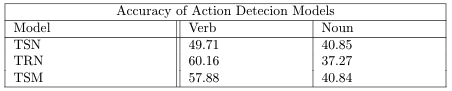
\includegraphics[scale=0.5]{imgs/action_detection_accuracy.png}
    \caption{Accuracy of action detection models (TSN, TSM, and TRN) for both verb classification and noun classification}
    \label{fig:chartForEvalActionDetection}
\end{figure}

As you know, the action detection system gives the best verb and Top 5 nouns. Thus, the evaluation program checked if the predicted best verb is equal to the answer verb when calculating the accuracy of verb classification, where the evaluation program checked if the answer noun is contained in the Top 5 nouns for evaluating the noun classification. As you could see in the figure \ref{fig:chartForEvalActionDetection}, the average accuracy of verb classification is higher than the average accuracy of noun classification, even though the system returns Top 5 nouns. Henceforth, it was decided to give more points to the detected verbs than the detected nouns.

\subsubsection{Evaluation for the Video Summarisation system}

To test how far the system can reduce the length of the video, the Epic Kitchens dataset, which is used for training and testing the action detection system, is used. Basically, the compression method of the video summarisation system strongly depends on the accuracy of the action detection system, because the system looks for the verb changes when compressing the result. According to the \hyperlink{ref8}{D. Damen et al. [8]}, with the pretrained model, the accuracy of the verb classification is much higher when using the training set rather than using the testing set.

What I did for this section is, execute the video summarisation system with videos in Epic Kitchens training set (dataset that is used for training the action detection system) and testing set (dataset that is used for testing the action detection system). The main reason of evaluating the system with both training set and testing set is because \hyperlink{ref8}{D. Damen et al. [8]} stated that for the verb classification with the pre-trained model, the accuracy when using the training set is about 8\% higher than the accuracy when using the testing set. It would be worth checking if this matters to the performance of the video summarisation system, so I planned to evaluate the compression rate by comparing the average compression rate of video summarisation with the training set and testing set. After running the video summarisation system, the original length of the video and the length of the summarised video were recorded in the CSV file. Then, by using those results, the compression rate was calculated using the following equation.

\[compression\_rate = len(result\_of\_summarisation) / len(original\_video)\]

The following table shows the min, max, and average compression rates for both training set and testing set of Epic Kitchens dataset. As you could see, the average compression rate of the training set is 0.254, where the average compression rate of the testing set is 0.309. Therefore, it would be possible to say that the more accurate the result of the action detection system, the better the video summarisation system could perform.

\begin{figure}[H]
    \centering
    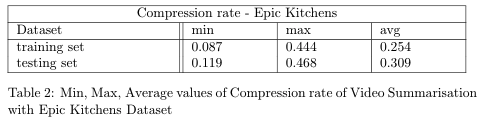
\includegraphics[scale=0.7]{imgs/compression_rate.png}
    \label{fig:compression_rate_table_EpicKitchens}
\end{figure}

As you could see in the table above, the highest compression rate is about 45\%. The main reason the high compression rate is because the video summarisation system that I designed is not able to compress the video if the same scenes (or same actions) are repeated. For example, if a person takes a cup, washes the cup, puts it back to the table, and does the same thing several times, then the system that I designed is not able to summarise this properly. Unfortunately, I was not able to find and implement solutions that could solve this issue. If I found a suitable solution and implemented it, probably, then the performance of the video summarisation system would be much better than the current version.

To evaluate the video summarisation system properly, the generated result (summarised texts) should be compared with the annotations or text recipes. Unfortunately, however, the Epic Kitchens dataset does not provide the text recipes of the cooking videos. Since there is no recipes to compare, I was not able to validate the generated texts.


\subsection{Discussion}

\subsubsection{Impact}

This project proposes a novel model for the video summarisation. This system performs object detection and action detection to extract data from video frames, and merge and compress the extracted data to summarise the given video. The video summarisation system that I proposed reads and parses the intermediate results of the object detection system and action detection system to merge the results, and compress the merged results to summarise the video. In other words, the strong point of the design of this video summarisation system is that the user could use and compose different pairs of action detection model and object detection model. This means that the user could replace the action detection model (Epic Kitchens models) or object detection model (YOLOv3) with other models. For example, you could replace the YOLOv3 model with \hyperlink{ref8}{EfficientDet [25]} or other object detection models, if you could make the new model to generate intermediate file with same format. As I mentioned in the evaluation section, the action detection system would not work properly if the point of view of the target video is different from the viewpoint of the videos that are used for training the action detection model. Thus, by replacing the action detection model with suitable model, you would be able to improve the accuracy of the results.

\subsubsection{Future Work and Improvements}

There are several points that could be improved in the future.\newline

\textbf{Object detection system}

When searching for the dataset to retrain the YOLOv3 model, I found that none of the dataset provides the images for the ingredients of the foods. Most of the datasets that contains the images about foods only have images of actual foods and dishes. Clearly, it would be possible to improve the performance of video summarisation system by making object detection system to detect ingredients in the video frames.

Furthermore, I found that the YOLOv3 model cannot recognise the processed food ingredients properly. For example, the YOLOv3 could recognise carrots, however, it cannot recognise the chopped carrots. Definitely, many ingredients were processed and transformed in the cooking videos. To summarise the cooking videos correctly, the techniques that helps the system to recognise the processed food ingredients should be invented.\newline\newline

\textbf{Action detection system}

For the action detection system, the location of the camera and sensors are important. This means that if the action detection models are trained with the video dataset in third person vision, then the action detection models would not be able to classify actions correctly with the videos in first person vision. The Epic Kitchens, which is used for training and testing the action detection system, is a dataset in first person vision. In other words, the video summarisation system might not work properly with videos in third person vision. I think it might be worth to train action detection models with other datasets that contain third person vision videos, and compare the performance of those new models with the Epic Kitchens pretrained models.\newline

\textbf{NLP methods in the merging process}

Also, the natural language processing functions that I implemented for filtering the irrelevant words from the results could be further improved. In the current version, I simply calculate the threshold value by dividing the maximum similarity value with 2. Probably, this might be too straightforward. If it is possible to improve the filtering method, the system would be able to generate much clear result texts.\newline

\section{Conclusion}

The video summarisation system that I designed uses the object detection and action recognition models to extract information from video frames. The object detection system can detect objects and classify objects. Similarly, the action detection system can recognise action in the given video frames, and classify verbs and nouns for the given action. The results of object detection system and action detection system are merged by filtering irrelevant words by calculating similarity values with wordnet. After merging the results, the system compresses the merged results to summarise the contents of the video. When compressing the results, the system checks if there are any meaningful changes by comparing the verbs, nouns, and objects. The average compression rate that is calculated by evaluating the video summarisation system is reasonably small, which means that the system could compress the results of detection properly.

However, it is hard to say that the system could filter all irrelevant words by calculating similarity values with wordnet. The final result texts still contain some irrelevant words, which makes the summarisation system confuse when compressing the results. Furthermore, as I mentioned in the evaluation section, the compression component cannot handle the repeating actions. Although it would be difficult to say that the summarised texts are accurate, since I did not validate the generated summary text files because I did not have the text recipes to compare with.

By doing this project, I was able to learn how to use and train the YOLOv3 model. Also, I learned many testing methods for the classification models. Furthermore, I was able to experience natural language processing methods by using wordnet.

\newpage

\section{References}
\hypertarget{ref1}{[1]} Forbes, "Video Marketing In 2018 Continues To Explode As Way To Reach Customers" [online]. Available :  \href{https://www.forbes.com/sites/tjmccue/2018/06/22/video-marketing-2018-trends-continues-to-explode-as-the-way-to-reach-customers}{https://www.forbes.com/sites/tjmccue/2018/06/22/video-marketing-2018-trends-continues-to-explode-as-the-way-to-reach-customers}
\newline
\hypertarget{ref2}{[2]} J. Redmon, A. Farhadi, "YOLOv3 : An Incremental Improvement", 2015. [online]. Available :  \url{https://pjreddie.com/media/files/papers/YOLOv3.pdf}
\newline
\hypertarget{ref3}{[3]} M. Otani, Y. Nakashima, E. Rahtu, J. Heikkila, N. Yokoya, "Video Summarization using Deep Semantic Features", 2016. [online]. Available : \url{https://arxiv.org/abs/1609.08758}
\newline
\hypertarget{ref4}{[4]} Y. Matsuda, H. Hoashi, K. Yanai, "UEC FOOD 100": 100-kind food dataset", 2012. [online]. Available : \url{http://foodcam.mobi/dataset100.html}
\newline
\hypertarget{ref5}{[5]} J. Redmon, A. Farhadi, "How to download and install the DarkNet", 2015. [online]. Available :  \url{https://pjreddie.com/darknet/install/}
\newline
\hypertarget{ref6}{[6]} M. Otani, Y. Nakashima, E. Rahtu, J. Heikkila, "Rethinking the Evaluation of Video Summaries", 2019. [online]. Available :  \url{https://arxiv.org/abs/1903.11328}
\newline
\hypertarget{ref7}{[7]} R. Fisher, "Edinburgh Utensils dataset", 2013. [online]. Available :  \url{http://homepages.inf.ed.ac.uk/rbf/UTENSILS/}
\newline
\hypertarget{ref8}{[8]}  D. Damen, S. Fidler, G. M. Farinella, D. Moltisanti, M. Wray, H. Doughty, T. Perrett, W. Price, E. Kazakos, J. Munro, A. Furnari, "Epic Kitchens", 2019. [online]. Available :  \url{https://epic-kitchens.github.io/2019}
\newline
\hypertarget{ref9}{[9]}  K. He, X. Zhang, S. Ren, J. Sun, "Deep residual learning for image recognition", 2016. [online] Available : \url{http://openaccess.thecvf.com/content_cvpr_2016/html/He_Deep_Residual_Learning_CVPR_2016_paper.html}
\newline
\hypertarget{ref10}{[10]}  S. Antol, A. Agrawal, J. Lu, M. Mitchell, D. Batra, C. L. Zitnick, D. Parikh, "VQA: Visual Question Answering", 2015. [online] Available : \url{http://openaccess.thecvf.com/content_iccv_2015/html/Antol_VQA_Visual_Question_ICCV_2015_paper.html}
\newline
\hypertarget{ref11}{[11]}  A. Karpathy, L. Fei-Fei, "Deep Visual-Semantic Alignments for Generating Image Descriptions", 2015. [online] Available : \url{https://www.cv-foundation.org/openaccess/content_cvpr_2015/html/Karpathy_Deep_Visual-Semantic_Alignments_2015_CVPR_paper.html}
\newline
\hypertarget{ref12}{[12]}  D. Damen, S. Fidler, G. M. Farinella, D. Moltisanti, M. Wray, H. Doughty, T. Perrett, W. Price, E. Kazakos, J. Munro, A. Furnari, "Scaling Egocentric Vision: The EPIC-KITCHENS Dataset", 2018. [online]. Available :  \url{https://arxiv.org/abs/1804.02748}
\newline
\hypertarget{ref13}{[13]} B. Zhou, A. ANdonian, A. Oliva, A. Torralba, "Temporal Relational Reasoning in Videos", 2017. [online]. Available :  \url{http://relation.csail.mit.edu/}
\newline
\hypertarget{ref14}{[14]} Y. Wu, J. Lim, M. H. Yang, "Online Object Tracking", 2013. [online]. Available :  \url{https://www.cv-foundation.org/openaccess/content_cvpr_2013/html/Wu_Online_Object_Tracking_2013_CVPR_paper.html}
\newline
\hypertarget{ref15}{[15]} A. Kathuria, "YOLO\_v3\_tutorial\_from\_scratch", [online]. Available :  \url{https://github.com/ayooshkathuria/YOLO_v3_tutorial_from_scratch}
\newline
\hypertarget{ref16}{[16]} L. Wang, Y. Xiong, Z. Wang, Y. Qiao, D. Lin, X. Tang, L. V. Gool, "Temporal Segment Networks for Action Recognition in Videos", [online]. Available :  \url{https://arxiv.org/abs/1705.02953}
\newline
\hypertarget{ref17}{[17]} J. Lin, C. Gan, S. Han, "TSM: Temporal Shift Module for Efficient Video Understanding", [online]. Available :  \url{https://arxiv.org/abs/1811.08383}
\newline
\hypertarget{ref18}{[18]} O. Utsumi, K. Miura, I. Ide, S. Sakai, H. Tanaka, "An object detection method for describing soccer games from video", [online]. Available :  \url{https://ieeexplore.ieee.org/abstract/document/1035714}
\newline
\hypertarget{ref19}{[19]} X. Yu, C. Xu, Q. Tian, H. w. Leong, "A ball tracking framework for broadcast soccer video", 2003. [online]. Available :  \url{https://www.researchgate.net/publication/4028111_A_ball_tracking_framework_for_broadcast_soccer_video}
\newline
\hypertarget{ref20}{[20]} P. Jodoin, Y. Benezeth, Y. Wang, "Meta-tracking for video scene understanding", 2013. [online]. Available :  \url{https://ieeexplore.ieee.org/abstract/document/6636607}
\newline
\hypertarget{ref21}{[21]} M. Murugavel, "YOLO-Annotation-Tool", 2013. [online]. Available :  \url{https://github.com/ManivannanMurugavel/YOLO-Annotation-Tool}
\newline
\hypertarget{ref22}{[22]} G. Bradski, "OpenCV video capture from file fails - github issue for opencv-python", [online]. Available : \url{https://github.com/ContinuumIO/anaconda-issues/issues/121}
\newline
\hypertarget{ref23}{[23]} ffmpeg Developers, "ffmpeg tool", 2016. [Software]. Available : \url{http://ffmpeg.org/}
\newline
\hypertarget{ref24}{[24]} G. A. Miller, "WordNet: a lexical database for English", 1995. [online]. Available : \url{https://dl.acm.org/doi/abs/10.1145/219717.219748}
\newline
\hypertarget{ref25}{[25]} M. Tan, R. Pang, Q. V. Le, "EfficientDet: Scalable and Efficient Object Detection", 2019. [online]. Available : \url{https://arxiv.org/abs/1911.09070}
\newline

\newpage

\section{Appendix}

\subsection{Installation}

TODO - 1. How to install python libraries  2. How to download source codes \& weights files from github repo

\subsection{Environments}

Due to the COVID-19, I had to leave UK. Thus, I was not able to test the final source codes in the lab machines. All codes (final version) were tested on the MacOS mojave.

\subsection{Instructions}

TODO - How to run programs ????

\subsection{Technologies Used}

\subsubsection{YOLOv3}

To implement the object detection system, PyTorch and OpenCV were used.

\textbf{1. PyTorch}

To implement the YOLOv3 model with Python language, the PyTorch was used. The PyTorch is a Python package that provides two high-level features, which are 1) computation of tensor with strong GPU acceleration, and 2) implementing deep neural networks built on a tape-based autograd system. PyTorch provides simple and straightforward APIs, so that the programmers could implement deep nerual networks easily and fastly.

\textbf{2. OpenCV}

The OpenCV is an open-sourced library that provides various functions and tools for Computer Vision. Unlike OpenCV C/C++ libarary, the opencv-python is easy to install and use. By using the pip (a package manager for python language), it could be installed in all macOS, Windows, and Linux. In this project, the OpenCV was used for various tasks such as reading video frames, getting the fps of the target video, data augmentation, and converting the color space of video frames.

\subsubsection{Action Detection System}

To implement the action detection system, PyTorch Hub and scikit-video were used.

\textbf{1. PyTorch Hub}

\hypertarget{actionDetection_used}{The PyTorch Hub} is a simple API and workflow the provides the basic building blocks for improving machine learning research reproducibility. The PyTorch Hub consists of a pre-trained model repository designed specifically to facilitate research reproducibility.  Therefore, by using the PyTorch Hub, researchers in various fields could easily discover each other’s research, leverage it as a baseline and build new cutting edge research from there. By using the PyTorch Hub, the system will download the pretrained action detection models.

\textbf{2. scikit-video}

The scikit-video is a python library that provides functions and tools for processing video files. Especially, the skvideo.io module, which was used for fixing the codec issue of the opencv-python, is created for using a FFmpeg/LibAV backend to read and write videos. So, by using the FFmpeg command line tool as a backend, the scikit-video library made it possible to process the video files that uses codecs or encoding methods that are not supported by the opencv-python library.

\end{document}
